\chapter{Benchmarking y análisis de complejidad asintótica}

\section{Análisis teórico}

\begin{table}[H]
  \centering
  \caption{Complejidad asintótica de operaciones}
  \begin{tabular}{@{}lccc@{}}
    \toprule
    \textbf{Operación} & \textbf{Peor caso} & \textbf{Promedio} & \textbf{Amortizado} \\
    \midrule
    \texttt{Search} & $\bigO(\log n)$ & $\bigO(\log n)$ & $\bigO(\log n)$ \\
    \texttt{Insert} & $\bigO(n)$ & $\bigO(\log n)$ & $\bigO(\log n)$ \\
    \texttt{Delete} & $\bigO(n)$ & $\bigO(\log n)$ & $\bigO(\log n)$ \\
    \texttt{InOrder} & $\bigO(n)$ & $\bigO(n)$ & $\bigO(n)$ \\
    \bottomrule
  \end{tabular}
\end{table}

\section{Resultados experimentales}

Entorno: Windows, amd64, Intel Core i7-13620H. Comando: \texttt{go test -bench=Benchmark -benchmem -count=3}. Parámetro $\alpha = 2/3$.

\begin{table}[H]
  \centering
  \caption{BenchmarkInsert (1000 inserciones por iteración)}
  \begin{tabular}{@{}rrrrr@{}}
    \toprule
    \textbf{Ejec.} & \textbf{iter.} & \textbf{ns/op} & \textbf{B/op} & \textbf{allocs/op} \\
    \midrule
    1 & 745 & 1\,631\,404 & 786\,557 & 9\,861 \\
    2 & 739 & 1\,448\,963 & 786\,548 & 9\,861 \\
    3 & 826 & 1\,631\,904 & 786\,548 & 9\,861 \\
    \midrule
    \textbf{Prom.} & --- & $\sim$1\,570\,757 & $\sim$786\,551 & 9\,861 \\
    \bottomrule
  \end{tabular}
\end{table}

\begin{table}[H]
  \centering
  \caption{BenchmarkSearch ($n = 10^5$ nodos previos)}
  \begin{tabular}{@{}rrrrr@{}}
    \toprule
    \textbf{Ejec.} & \textbf{iter.} & \textbf{ns/op} & \textbf{B/op} & \textbf{allocs/op} \\
    \midrule
    1 & 5\,352\,201 & 218.2 & 0 & 0 \\
    2 & 5\,656\,558 & 207.8 & 0 & 0 \\
    3 & 5\,320\,170 & 216.0 & 0 & 0 \\
    \midrule
    \textbf{Prom.} & --- & $\sim$214 & 0 & 0 \\
    \bottomrule
  \end{tabular}
\end{table}

\begin{table}[H]
  \centering
  \caption{BenchmarkDelete (1000 inserciones + 1000 eliminaciones)}
  \begin{tabular}{@{}rrrrr@{}}
    \toprule
    \textbf{Ejec.} & \textbf{iter.} & \textbf{ns/op} & \textbf{B/op} & \textbf{allocs/op} \\
    \midrule
    1 & 750 & 1\,669\,327 & 803\,636 & 9\,875 \\
    2 & 771 & 1\,623\,863 & 803\,638 & 9\,875 \\
    3 & 832 & 1\,515\,044 & 803\,636 & 9\,875 \\
    \midrule
    \textbf{Prom.} & --- & $\sim$1\,602\,745 & $\sim$803\,637 & 9\,875 \\
    \bottomrule
  \end{tabular}
\end{table}

\begin{figure}[H]
  \centering
  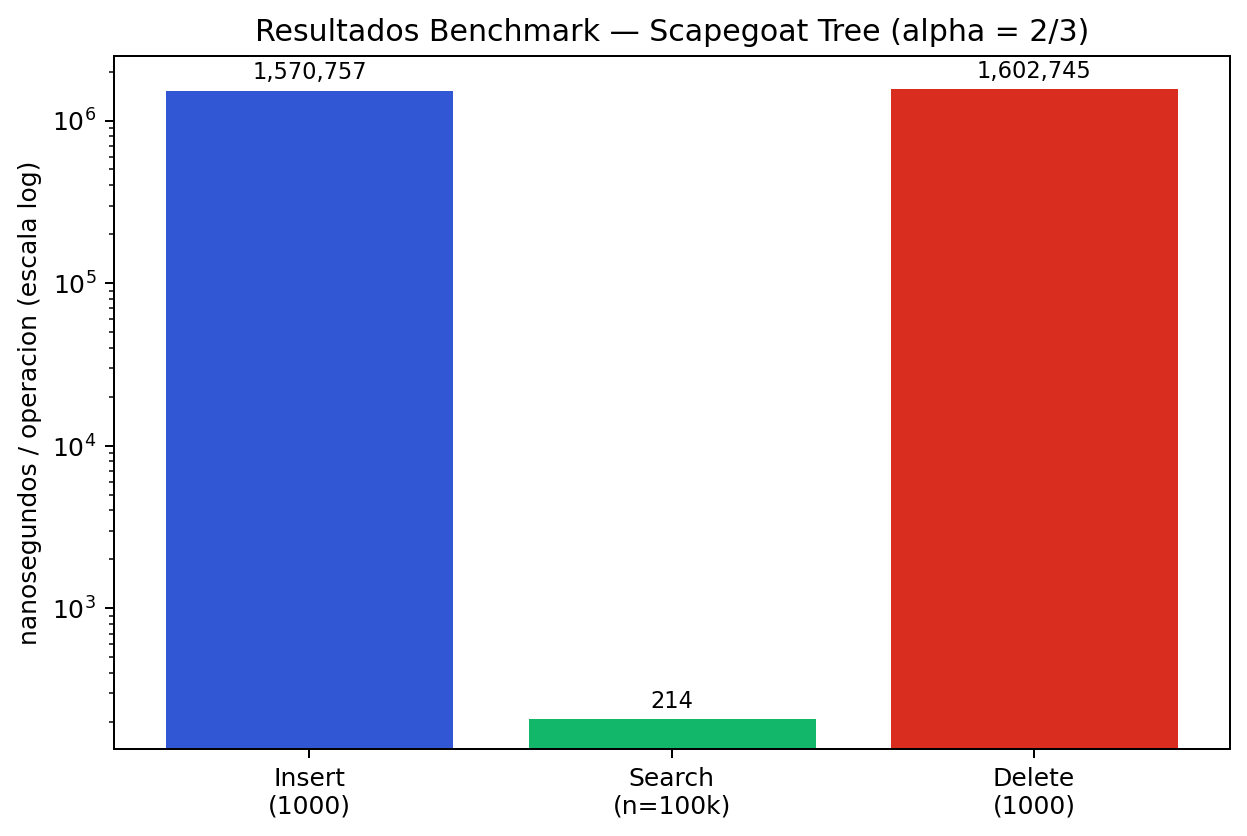
\includegraphics[width=0.78\textwidth]{diagrams/04-benchmark.png}
  \caption{Comparativa de benchmarks (escala logarítmica)}
  \label{fig:benchmark}
\end{figure}

\begin{figure}[H]
  \centering
  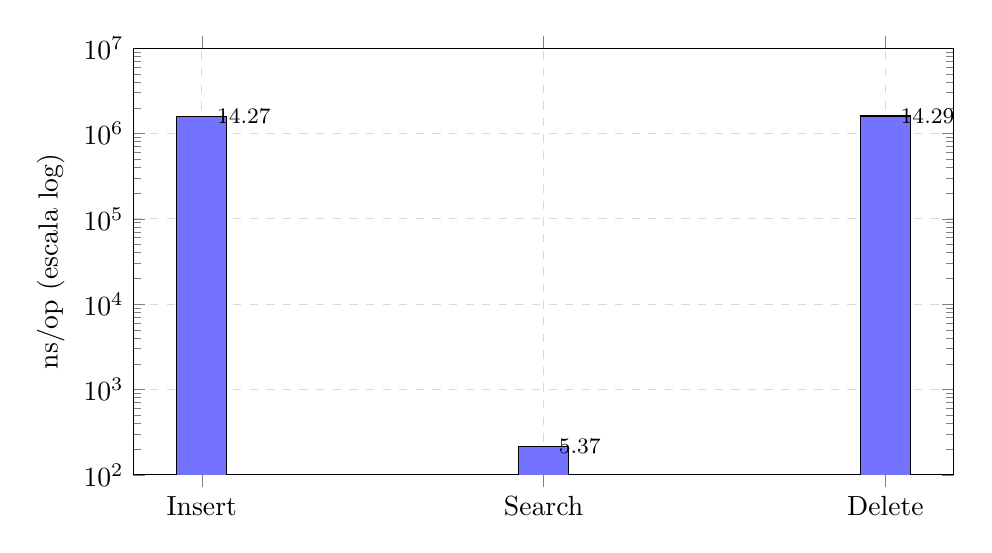
\begin{tikzpicture}
    \begin{axis}[
      ybar,
      bar width=18pt,
      width=12cm,
      height=7cm,
      ylabel={ns/op (escala log)},
      ymode=log,
      symbolic x coords={Insert, Search, Delete},
      xtick=data,
      ymin=100,
      ymax=10000000,
      nodes near coords={\pgfmathprintnumber\pgfplotspointmeta},
      every node near coord/.append style={font=\footnotesize, anchor=west, xshift=2pt},
      grid=major,
      grid style={dashed,gray!30},
      scaled y ticks=false
    ]
      \addplot[fill=blue!55] coordinates {(Insert,1570757) (Search,214) (Delete,1602745)};
    \end{axis}
  \end{tikzpicture}
  \caption{Gráfico de barras --- tiempos promedio por operación}
  \label{fig:benchmark-bars}
\end{figure}

\section{Interpretación}

La búsqueda exhibe $\sim 4.7 \times 10^6$ ops/s con cero asignaciones de heap. Insert y Delete muestran picos por reconstrucciones; la envolvente superior de inserción ordenada crece más rápido que en secuencias aleatorias, confirmando la teoría del scapegoat.
